\section{Theorie}
\label{sec:Theorie}
Ziele dieses Versuches sind die Bestimmung von Brennweiten $f$ verschiedener
Linsen und Linsensysteme, mitunter nach den Methoden von Bessel und Abbe, sowie
die Verifizierung des Abbildungsgesetzes und der Linsengleichung.

Linsen sind Objekte optisch dickeren Mediums als ihre Umgebung, die Lichtstrahlen
nach dem Brechungsgesetz brechen. Es wird zwischen bündelnden konvexen Sammellinsen
mit jeweils positiver Brennweite $f$ und Bildweite $b$, die ein reelles Bild erzeugen,
und zerstreuenden, konkaven Streulinsen mit jeweils negativen $f$ und $b$, die
ein virtuelles Bild erzeugen, unterschieden.

In Abbildung \ref{fig:bild1} sind die Bildkonstruktionen beider Linsentypen dargestellt.

\begin{figure} [H]
    \centering
    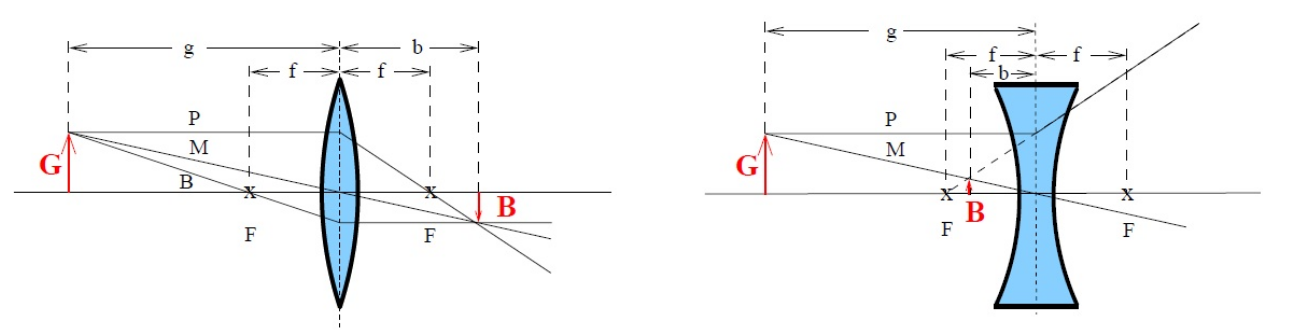
\includegraphics[scale=0.35]{content/bild1.png}
    \caption{Bildkonstruktionen einer Sammel- (rechts) und Streulinse (links) [1]}
    \label{fig:bild1}
  \end{figure}

  Für dicke Linsen kann nicht mehr davon ausgegangen werden, dass die Brechung in der Mittelebene
  stattfindet. Stattdessen werden zwei Hauptebenen $H$, $H'$ betrachtet, an denen Brechung stattfindet
  (s. Abbildung \ref{fig:bild2}).

  \begin{figure} [H]
    \centering
    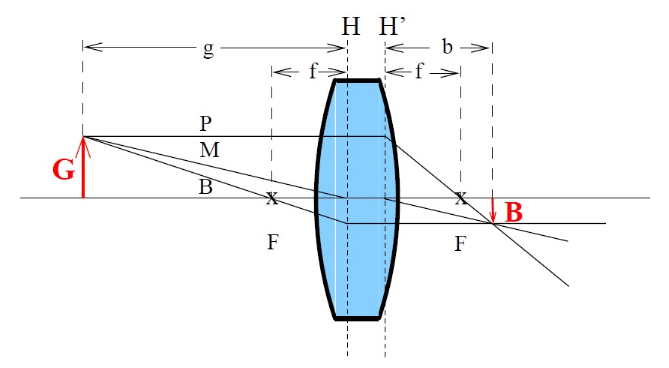
\includegraphics[scale=0.35]{content/bild2.png}
    \caption{Bildkonstruktionen einer dicken Sammellinse [1]}
    \label{fig:bild2}
  \end{figure}

  Die ausgezeichneten Strahlen, die in der Bildkonstruktion betrachtet werden, sind
  der Mittelpunktsstrahl M, der Brennpunktsstrahl B und der Parallelstrahl P.
  Die beiden letzteren wandeln sich an der Brechebene in den jeweils anderen.

  Es gelten außerdem das Abbildungsgesetz 

  \begin{equation}
      V = \frac{B}{G} = \frac{b}{g}
      \label{eqn:abbgesetz}
  \end{equation}

  mit der Bildgröße $B$, Gegenstandsgröße $G$ und Gegenstandsweite $g$

  und für dünne Linsen die Linsengleichung

  \begin{equation}
      \frac{1}{f} = \frac{1}{b} + \frac{1}{g}
      \label{eqn:linsengl} \; .
  \end{equation}

Die Linsengleichung \eqref{eqn:linsengl} gilt auch für dicke Linsen, wenn $b$ und $g$
bezüglich der Hauptebenen bestimmt werden.

Des weiteren wird die optische Brechkraft $D$ definiert als

\begin{equation}
    D = \frac{1}{f} = \sum_i^N D_i
    \label{eqn:brechkraft}
\end{equation}

und summiert sich bei einem Mehrlinsensystem aus den jeweiligen Brechkräften $D_i$ auf.


Außerdem können verschiedene Abbildungsfehler auftreten. Zwei von ihnen sind
die sphärische Abberation, die darin besteht, dass sich die Brennweiten mittelachsennaher
und -ferner Strahlen unterscheiden, sowie die chromatische, nach der Lichtstrahlen verschiedener
Wellenlängen unterschiedlich stark gebrochen werden. Kurzwelliges Licht wird stärker gebrochen,
als langwelliges.

\subsection{Die Bessel-Methode}

Nach dieser Methoden bleibt der Abstand $e$ zwischen Gegenstand und Schirm konstant und
es werden die zwei Linsenpositionen ermittelt, bei denen das Bild scharf ist. Wie auch in 
Abbildung \ref{fig:bild3} dargestellt sind die Positionen symmetrisch und die Werte 
für $b$ und $g$ jeweils vertauscht.

Die Brennweite berechnet sich nach der Gleichung

\begin{equation}
    f = \frac{e^2 - d^2}{4e}
    \label{eqn:bessel}
\end{equation}

mit den Abständen 

\begin{align*}
    e &= g_1 + b_1 = g_2 + b_2 \\
    d &= |g_1 - b_1| = |g_2 - b_2| \; .
\end{align*}

\begin{figure} [H]
    \centering
    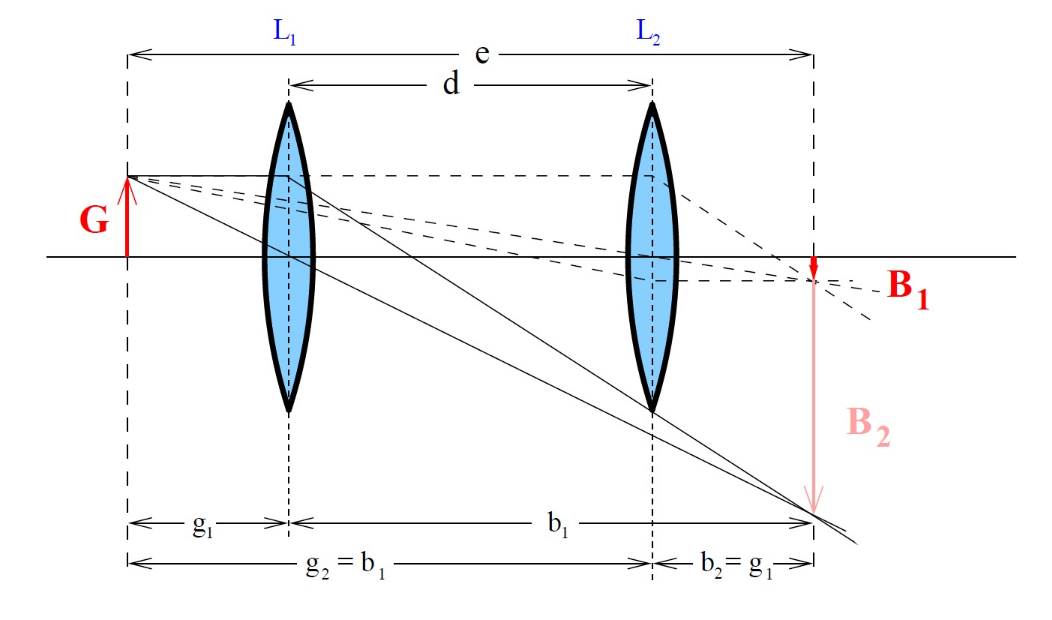
\includegraphics[scale=0.3]{content/bild3.png}
    \caption{Bildkonstruktionen der Bessel-Methode [1]}
    \label{fig:bild3}
  \end{figure}

  \subsection{Die Abbe-Methode}

  Diese Methode untersucht die Brennweite eines Linsensystems, bei dem zwischen Gegenstand
  und Sammellinse eine Streulinse justiert wird, wie in Abbildung \ref{fig:bild4}
  dargestellt. Der Abstand zwischen den Linsen soll dabei konstant bleiben.
  Auch hier wird die Position für ein scharfes Bild ermittelt und $b$, $g$ und $b'$, $g'$
  bezüglich eines Referenzpunktes A gemessen. 

  Die Brennweite $f$ kann dann aus den Gleichungen

  \begin{align}
      g' &= g + h = f \left( 1 + \frac{1}{V} \right) + h\label{eqn:abbe1}\\
      b' &= b + h' = f \left( 1 + V \right) + h'
      \label{eqn:abbe}
  \end{align}

  bestimmt werden.

  \begin{figure} [H]
    \centering
    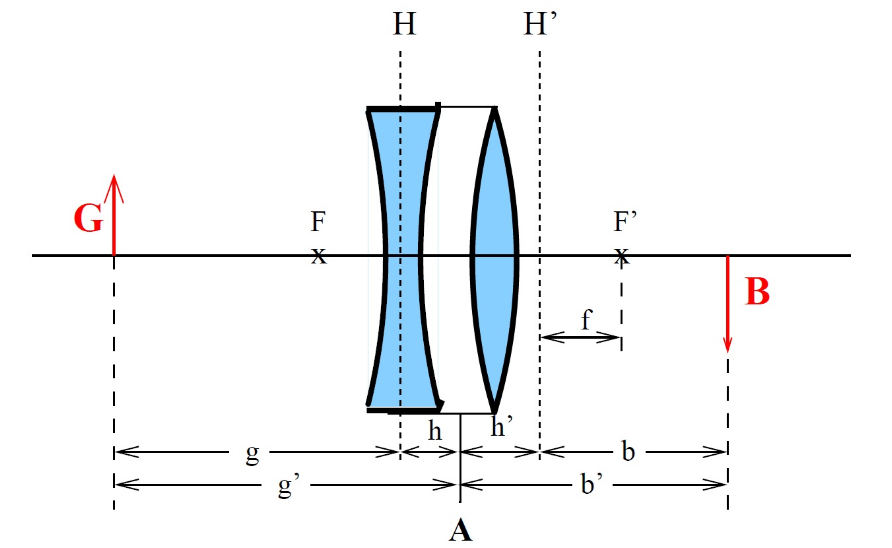
\includegraphics[scale=0.3]{content/bild4.png}
    \caption{Bildkonstruktionen der Abbe-Methode [1]}
    \label{fig:bild4}
  \end{figure}














